\documentclass[12pt]{article}

\usepackage{amsmath}
\usepackage{amssymb}
\usepackage[dvips]{graphicx}
\usepackage{eepic}
\usepackage{color}
\usepackage{wasysym} % \female \male
\usepackage[landscape,pdftex]{geometry}
\usepackage{fancyhdr}
\usepackage{hyperref}

\definecolor{cantelope}{rgb}{1.0,0.8,0.4}
\hypersetup{
    colorlinks, urlcolor={cantelope}
}
\hypersetup{pdfpagemode=UseNone} % don't show bookmarks on initial view

\DeclareOption{bigsym}{\DeclareSymbolFont{largesymbols}{OMX}{psycm}{m}{n}}
\ProcessOptions

\setlength{\oddsidemargin}{-0.75in}
\setlength{\evensidemargin}{-0.75in}
\setlength{\topmargin}{-1in}
\setlength{\textheight}{7.75in}
\setlength{\textwidth}{10.5in}
\setlength{\footskip}{0in}
\setlength{\parindent}{0pt}
\setlength{\rightskip}{0pt plus 1fil} % makes ragged right

\renewcommand{\familydefault}{phv} % helvetica

% following: color
\definecolor{mybgcolor}{rgb}{0,0,0.3125}
\definecolor{myyellow}{rgb}{1,1,0.4}
\definecolor{myblue}{rgb}{0.4,0.8,1}
\definecolor{mypink}{rgb}{1,0.4,1}
\definecolor{mywhite}{rgb}{1,1,1}

% header/footer layout
\pagestyle{fancy}
\lhead{} \chead{} \rhead{}
\lfoot{} \cfoot{} \rfoot{\color{myyellow} \thepage}
\renewcommand{\headrulewidth}{0pt}
\renewcommand{\footrulewidth}{0pt}

% font sizes
\newcommand{\superlarge}{\fontsize{60}{60} \selectfont}
\newcommand{\titlesize}{\fontsize{40}{50} \selectfont}
\newcommand{\headsize}{\fontsize{35}{35} \selectfont}
\newcommand{\textsize}{\fontsize{30}{35} \selectfont}
\newcommand{\smallsize}{\fontsize{25}{30} \selectfont}
\newcommand{\smallersize}{\fontsize{20}{25} \selectfont}
\newcommand{\smallestsize}{\fontsize{18}{22} \selectfont}
\newcommand{\lod}{\text{LOD}}
\newcommand{\plod}{\text{pLOD}}
\newcommand{\bic}{\text{BIC}}
\newcommand{\rss}{\text{RSS}}
\newcommand{\var}{\text{var}}
\newcommand{\M}{\text{M}}

\definecolor{citecolor}{rgb}{0.44,0.44,0.44}
\newcommand{\citesize}{\fontsize{14}{18} \selectfont}

% a few macros
\newcommand{\bi}{\begin{itemize}}
\newcommand{\bbi}{\vspace{24pt} \begin{itemize} \itemsep8pt}
\newcommand{\ei}{\end{itemize}}
\newcommand{\ig}{\includegraphics}
\newcommand{\subt}[1]{{\footnotesize \color{subtitle} {#1}}}
\newcommand{\ttsm}{\tt \small}
\newcommand{\ttfn}{\tt \footnotesize}
\newcommand{\figh}[2]{\centerline{\includegraphics[height=#2\textheight]{#1}}}
\newcommand{\figw}[2]{\centerline{\includegraphics[width=#2\textwidth]{#1}}}

\pagecolor{mybgcolor}
\color{mywhite}

\begin{document}
\thispagestyle{empty}

\begin{center}
\titlesize \color{myyellow}


\vspace*{15mm}

Multiparent populations \& R/qtl2

\color{mypink}
\rule{10in}{1mm}

\vspace{5mm}

\textsize \color{myblue}
Karl Broman
\vspace{5mm}

\color{mywhite}
{\smallsize Biostatistics and Medical Informatics

University of Wisconsin -- Madison
\vspace{20mm}


\href{http://kbroman.org/qtl2}{\tt kbroman.org/qtl2} \\[3pt]
\href{http://kbroman.org}{\tt kbroman.org} \\[3pt]
\href{https://github.com/kbroman}{\tt github.com/kbroman} \\
\href{https://twitter.com/kwbroman}{\tt @kwbroman} \\
}

\end{center}



\newpage


\headsize \color{myyellow}
\hfill \begin{minipage}{5.75in}
\centering
QTL mapping
\end{minipage}

\vspace{5mm}

\figh{Figs/lodcurve_insulin_with_effects.pdf}{0.9}

\newpage


\headsize \color{myyellow}
\hfill \begin{minipage}{5.75in}
\centering
Congenic line / NIL
\end{minipage}


\figw{Figs/congenic.pdf}{1.0}

\newpage



\headsize \color{myyellow}
\hfill \begin{minipage}{5.75in}
\centering
Improving precision
\end{minipage}


\vspace{3cm}

\color{mywhite} \smallsize

\hfill \begin{minipage}[t]{9.5in}
\begin{itemize}
\itemsep24pt
\setlength{\rightskip}{0pt plus 1fil} % makes ragged right
\item more recombinations
\item more individuals
\item more precise phenotypes
\item lower-level phenotypes
  \begin{itemize}
  \item[] {\color{myblue} \smallersize transcripts, proteins, metabolites}
  \end{itemize}
\end{itemize} \end{minipage}


\newpage



\headsize \color{myyellow}
\hfill \begin{minipage}{5.75in}
\centering
Advanced intercross lines
\end{minipage}

\vspace{5mm}

\figh{Figs/ail.pdf}{0.9}

\newpage


\headsize \color{myyellow}
\hfill \begin{minipage}{5.75in}
\centering
Recombinant inbred lines
\end{minipage}

\vspace{5mm}

\figh{Figs/rilines.pdf}{0.9}

\newpage



\headsize \color{myyellow}
\hfill \begin{minipage}{5.75in}
\centering
Recombinant inbred lines
\end{minipage}

\vspace{5mm}

\figh{Figs/riself.pdf}{0.9}

\newpage



\headsize \color{myyellow}
\hfill \begin{minipage}{6.75in}
\centering
Collaborative Cross/MAGIC
\end{minipage}

\vspace{5mm}

\figh{Figs/ri8.pdf}{0.9}


\newpage

\headsize \color{myyellow}
\hfill \begin{minipage}{5.75in}
\centering
Heterogeneous stock
\end{minipage}


\vspace{5mm}

\figh{Figs/hs.pdf}{0.9}


\newpage

\newpage

\headsize \color{myyellow}
\hfill \begin{minipage}{5.75in}
\centering
MAGIC lines
\end{minipage}

\vspace{20mm}

\centerline{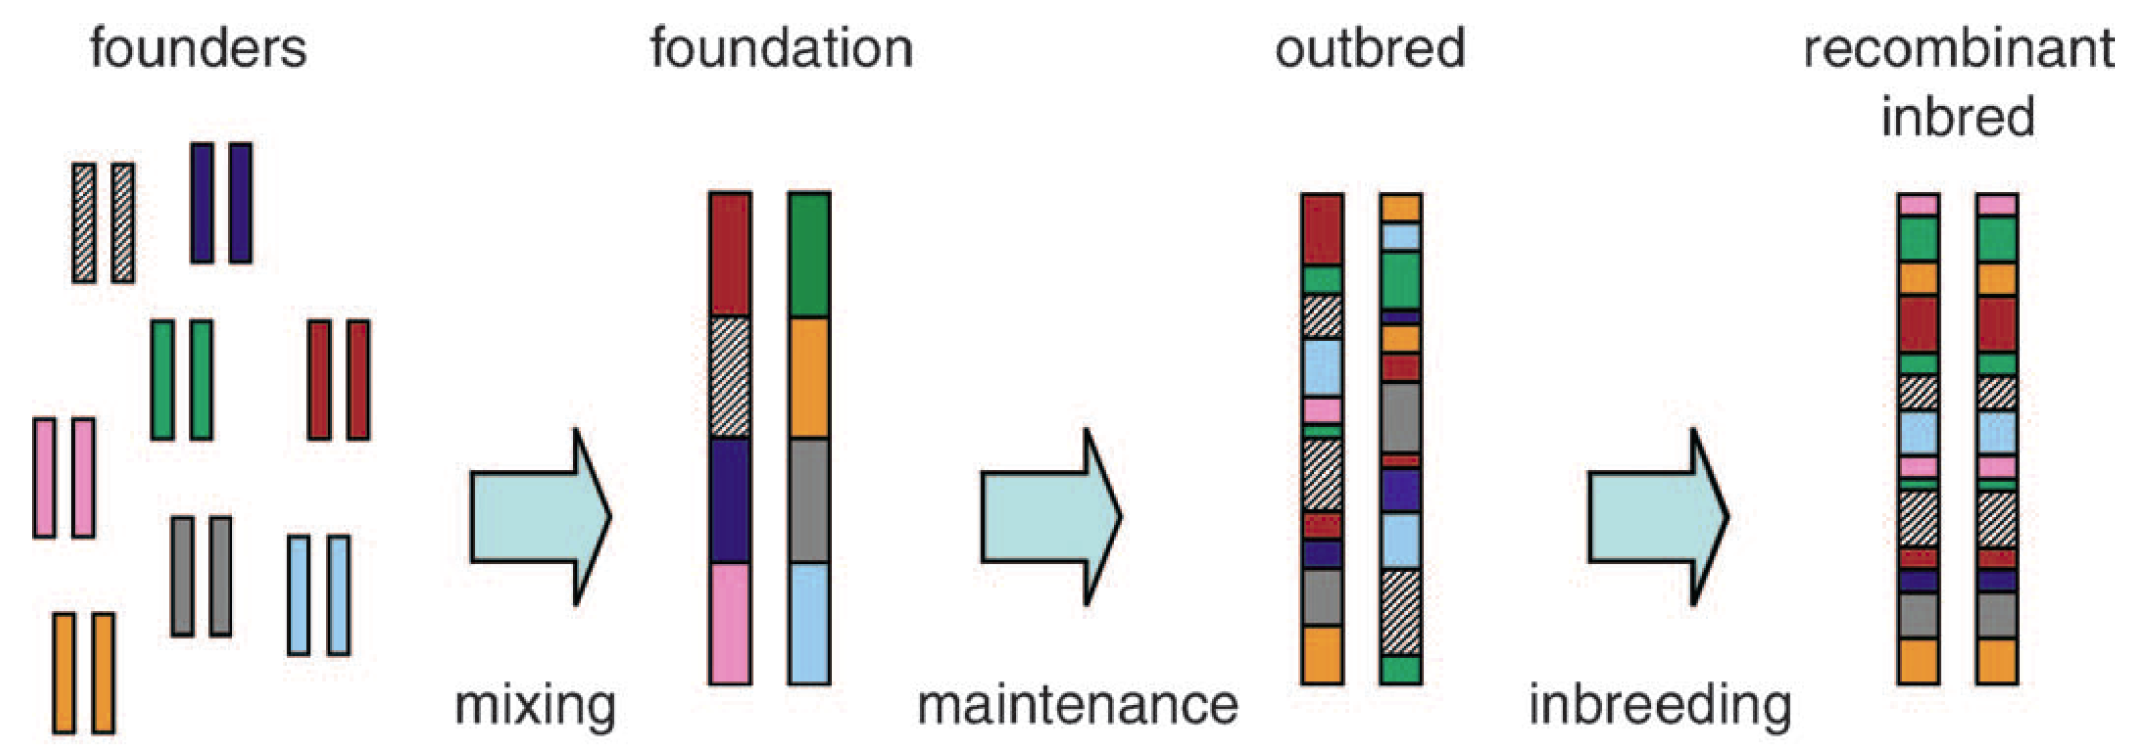
\includegraphics[width=10in]{Figs/valdar_genet2006.png}}

\smallsize \color{myyellow}
\hspace*{52mm} combine \hspace*{35mm} mix \hspace*{52mm} fix

\vfill

\hfill {\citesize \color{citecolor} \href{http://www.genetics.org/content/172/3/1783.full}{Valdar et al., Genetics 172:1783, 2006}}

\vspace*{5mm}

\newpage

\addtocounter{page}{-1}

\headsize \color{myyellow}
\hfill \begin{minipage}{5.75in}
\centering
MAGIC lines
\end{minipage}

\vspace{20mm}

\centerline{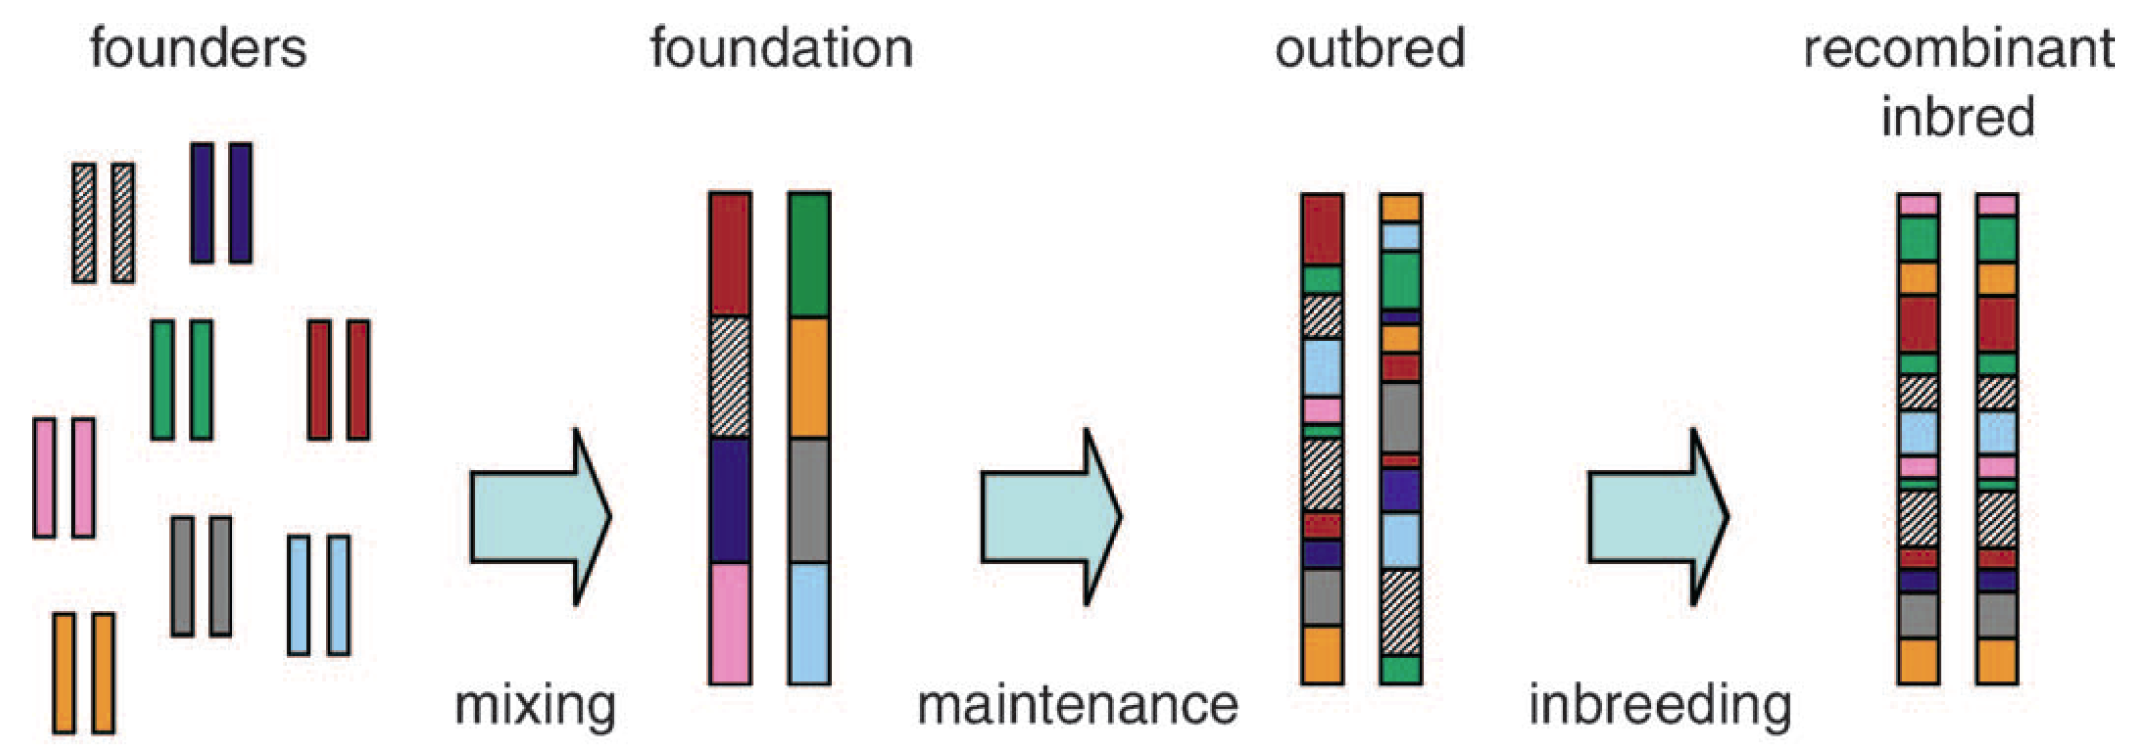
\includegraphics[width=10in]{Figs/valdar_genet2006.png}}

\smallsize \color{myyellow}
\hspace*{52mm} combine \hspace*{35mm} mix \hspace*{52mm} fix

\smallersize
\color{mywhite}
\vspace{20pt}

\hspace*{6mm}
\begin{minipage}[t]{45mm}
\vspace*{0mm}
\centering

How many? \\[20pt]

\end{minipage}
\hspace{57mm}
\begin{minipage}[t]{45mm}
\vspace*{0mm}
\centering


\end{minipage}
\hspace{18mm}
\begin{minipage}[t]{45mm}
\vspace*{0mm}
\centering


\end{minipage}


\vfill

\hfill {\citesize \color{citecolor} \href{http://www.genetics.org/content/172/3/1783.full}{Valdar et al., Genetics 172:1783, 2006}}

\vspace*{5mm}


\newpage

\addtocounter{page}{-1}

\headsize \color{myyellow}
\hfill \begin{minipage}{5.75in}
\centering
MAGIC lines
\end{minipage}

\vspace{20mm}

\centerline{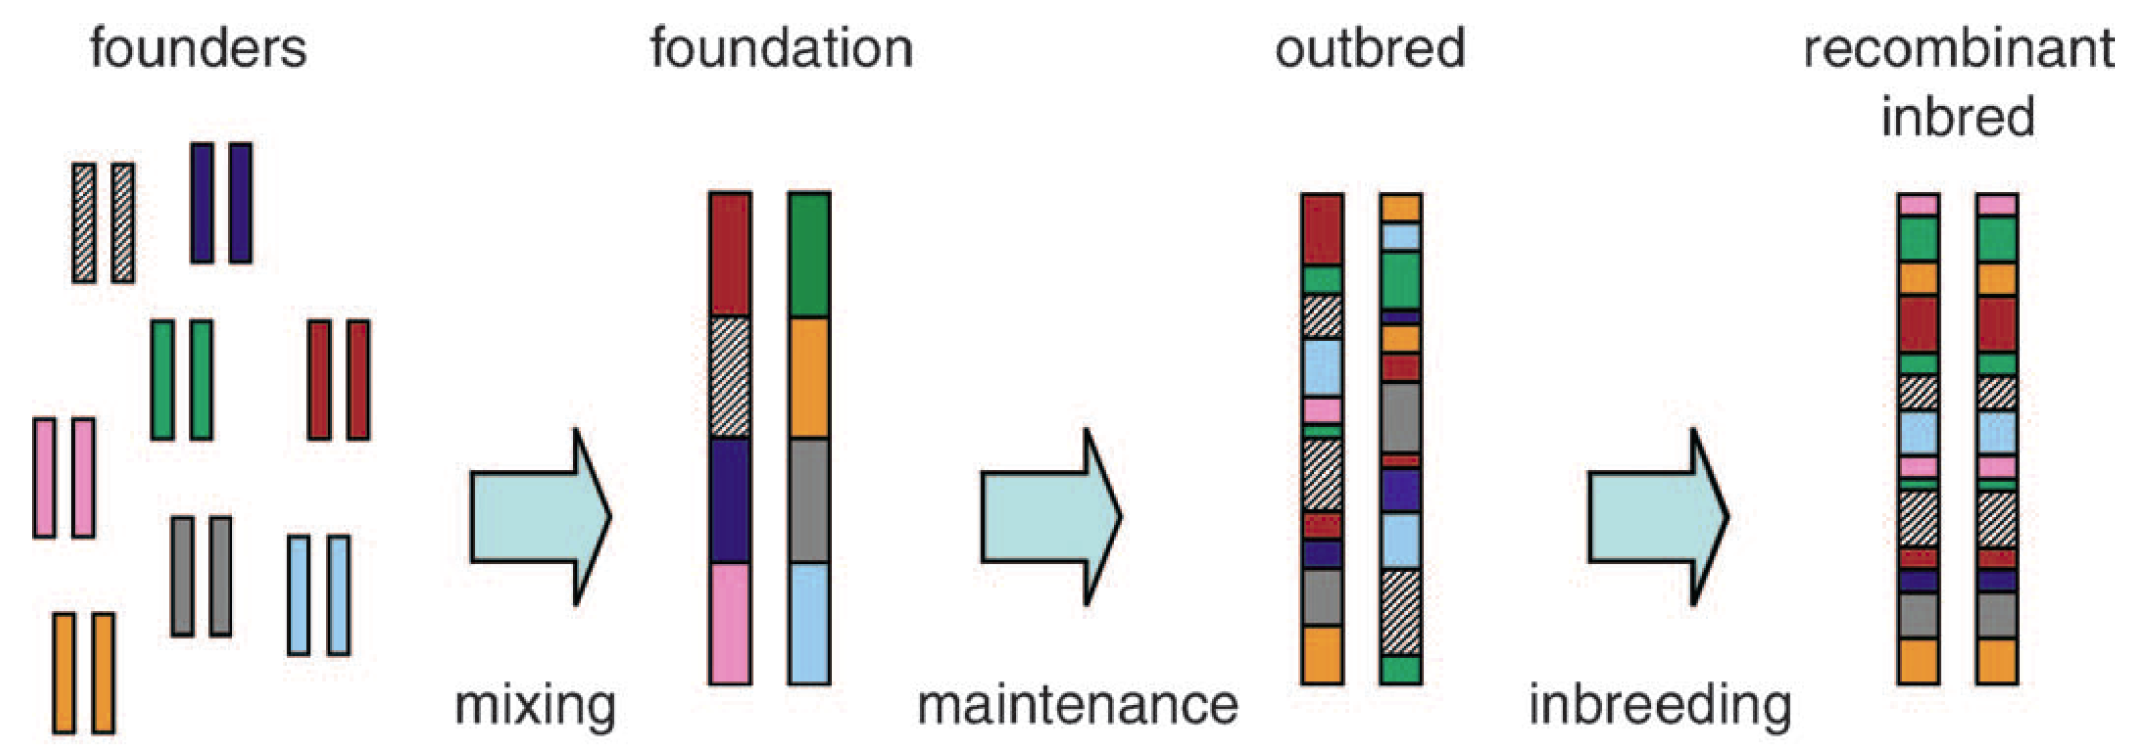
\includegraphics[width=10in]{Figs/valdar_genet2006.png}}

\smallsize \color{myyellow}
\hspace*{52mm} combine \hspace*{35mm} mix \hspace*{52mm} fix

\smallersize
\color{mywhite}
\vspace{20pt}

\hspace*{6mm}
\begin{minipage}[t]{45mm}
\vspace*{0mm}
\centering

How many? \\[20pt]
Which?
\end{minipage}
\hspace{57mm}
\begin{minipage}[t]{45mm}
\vspace*{0mm}
\centering

\end{minipage}
\hspace{18mm}
\begin{minipage}[t]{45mm}
\vspace*{0mm}
\centering


\end{minipage}


\vfill

\hfill {\citesize \color{citecolor} \href{http://www.genetics.org/content/172/3/1783.full}{Valdar et al., Genetics 172:1783, 2006}}

\vspace*{5mm}


\newpage

\addtocounter{page}{-1}

\headsize \color{myyellow}
\hfill \begin{minipage}{5.75in}
\centering
MAGIC lines
\end{minipage}

\vspace{20mm}

\centerline{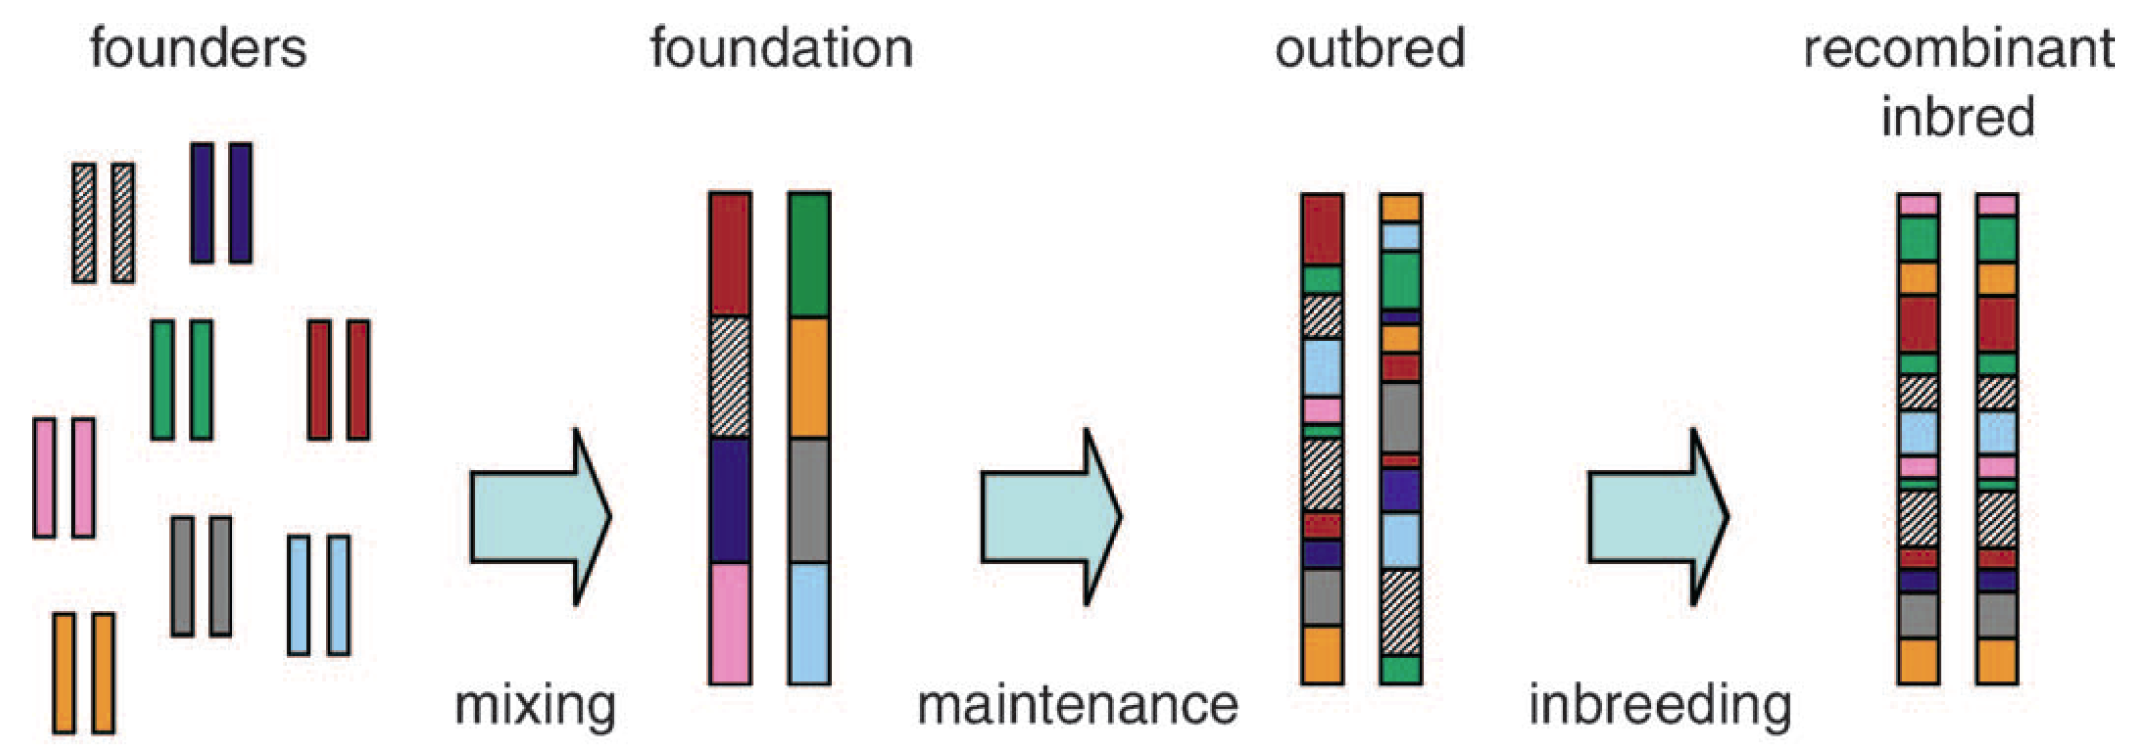
\includegraphics[width=10in]{Figs/valdar_genet2006.png}}

\smallsize \color{myyellow}
\hspace*{52mm} combine \hspace*{35mm} mix \hspace*{52mm} fix

\smallersize
\color{mywhite}
\vspace{20pt}

\hspace*{6mm}
\begin{minipage}[t]{45mm}
\vspace*{0mm}
\centering

How many? \\[20pt]
Which?
\end{minipage}
\hspace{57mm}
\begin{minipage}[t]{45mm}
\vspace*{0mm}
\centering

How long?
\end{minipage}
\hspace{18mm}
\begin{minipage}[t]{45mm}
\vspace*{0mm}
\centering


\end{minipage}


\vfill

\hfill {\citesize \color{citecolor} \href{http://www.genetics.org/content/172/3/1783.full}{Valdar et al., Genetics 172:1783, 2006}}

\vspace*{5mm}


\newpage

\addtocounter{page}{-1}

\headsize \color{myyellow}
\hfill \begin{minipage}{5.75in}
\centering
MAGIC lines
\end{minipage}

\vspace{20mm}

\centerline{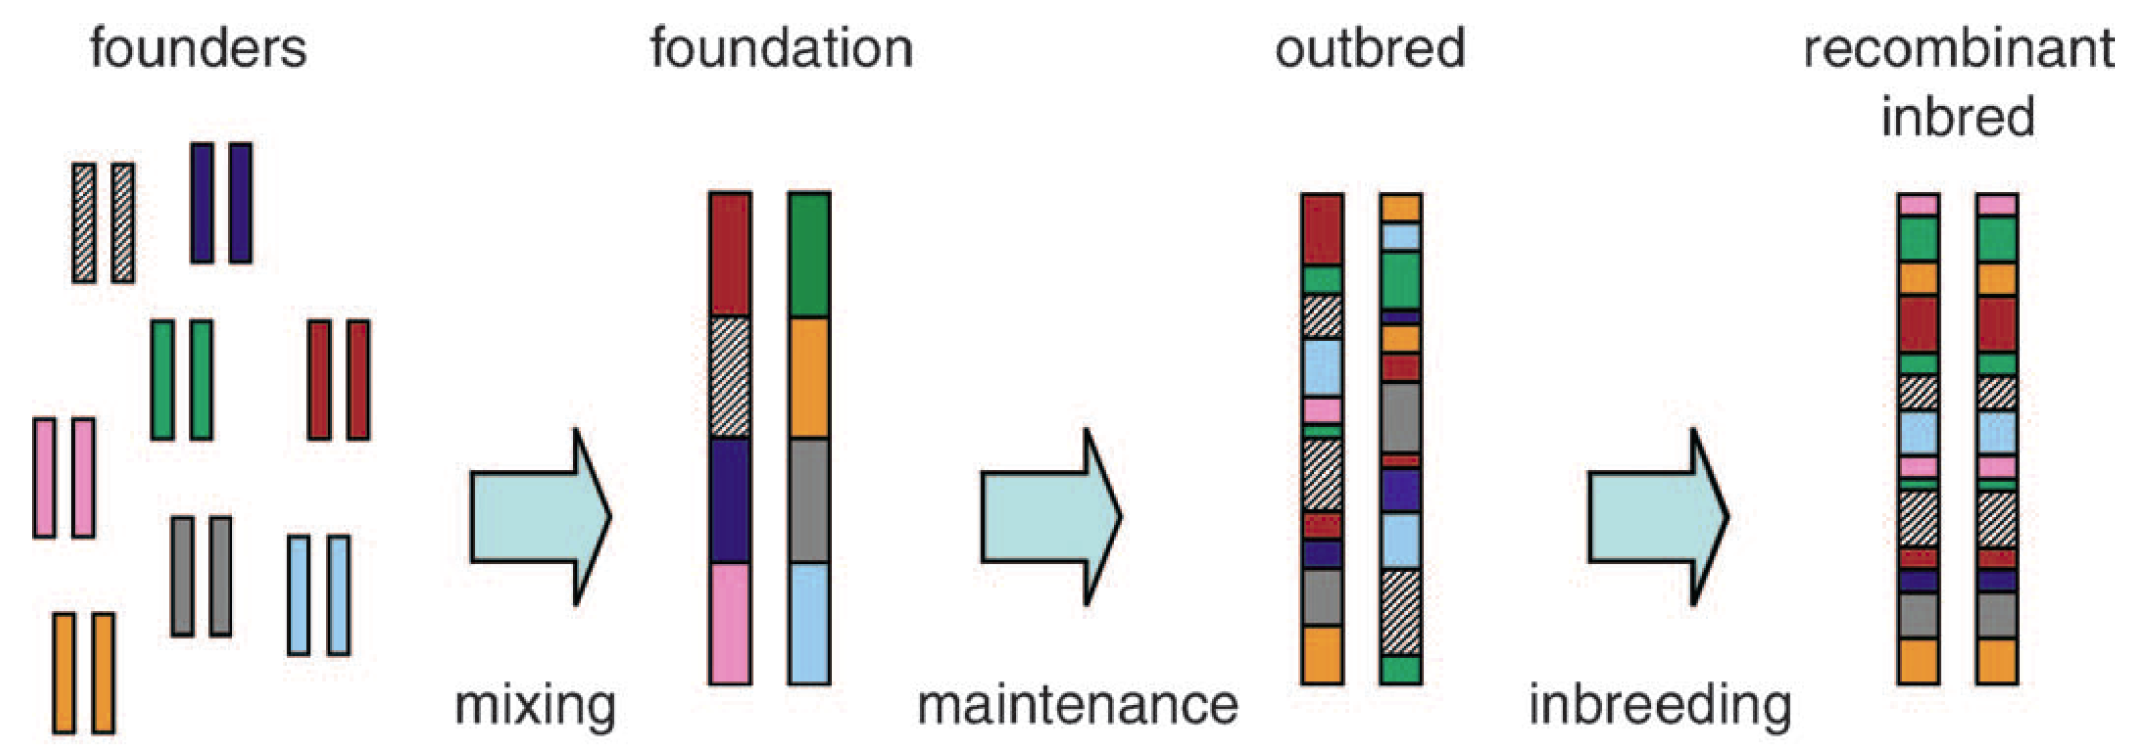
\includegraphics[width=10in]{Figs/valdar_genet2006.png}}

\smallsize \color{myyellow}
\hspace*{52mm} combine \hspace*{35mm} mix \hspace*{52mm} fix

\smallersize
\color{mywhite}
\vspace{20pt}

\hspace*{6mm}
\begin{minipage}[t]{45mm}
\vspace*{0mm}
\centering

How many? \\[20pt]
Which?
\end{minipage}
\hspace{57mm}
\begin{minipage}[t]{45mm}
\vspace*{0mm}
\centering

How long?
\end{minipage}
\hspace{18mm}
\begin{minipage}[t]{45mm}
\vspace*{0mm}
\centering

How?
\end{minipage}


\vfill

\hfill {\citesize \color{citecolor} \href{http://www.genetics.org/content/172/3/1783.full}{Valdar et al., Genetics 172:1783, 2006}}

\vspace*{5mm}



\newpage

\headsize \color{myyellow}
\hfill \begin{minipage}{5.75in}
\centering
MAGIC is magic
\end{minipage}

\vspace{25mm}

\color{mywhite}
\smallsize

\hfill \begin{minipage}{10in}
\begin{itemize}
\itemsep24pt
\item Genetic diversity

\item High-precision mapping

\item Predictable linkage disequilibrium

\item Phenotype replicates to reduce individual variation

\item Pool phenotypes from multiple labs, environments, treatments

\item Genotype once

\color{mybgcolor}
\item Cool name

\end{itemize}
\end{minipage}

\newpage

\addtocounter{page}{-1}

\headsize \color{myyellow}
\hfill \begin{minipage}{5.75in}
\centering
The goal
\end{minipage}

\vspace{25mm}

\color{mywhite}
\smallsize

\hfill \begin{minipage}{9.5in}
Identify QT{\color{mypink} G}
\end{minipage}

\vspace{15mm}

\hfill \begin{minipage}{9in}
\color{myblue}
\begin{itemize}
\itemsep24pt
\item Power
\item Mapping precision
\item Estimate QTL allele frequencies
\end{itemize}
\end{minipage}


\newpage


\headsize \color{myyellow}
\hfill \begin{minipage}{5.75in}
\centering
Principles
\end{minipage}

\vspace{25mm}

\color{mywhite}
\smallersize

\hfill \begin{minipage}{10in}
\begin{itemize}
\itemsep24pt
\item Avoid population structure
\item Tradeoff between {\color{myblue} power for \emph{de novo\/} discovery}
  and {\color{myblue} mapping precision}
\item More QTL to find $ \ \Rightarrow \ $ more QTL getting in the way?
\item More QTL alleles $ \ \Rightarrow \ $ less information about each
\item Are QTL alleles common or rare?
\end{itemize}
\end{minipage}



\newpage


\headsize \color{myyellow}
\hfill \begin{minipage}{5.75in}
\centering
How many founders?
\end{minipage}

\vspace{25mm}

\color{mywhite}
\smallersize

\hspace{0.5in} \begin{minipage}[t]{4.8in}
\vspace*{0mm}

\hspace*{0.5in} {\color{myblue} \smallsize More}

\vspace{6mm}

\begin{itemize}
\itemsep16pt
\item More general use
\item More QTL
\item Greater precision
\item Estimate allele frequencies
\item Haplotype analysis in founders
\end{itemize}

\end{minipage}
\hfill
\begin{minipage}[t]{4.8in}
\vspace*{0mm}

\hspace*{0.5in} {\color{myblue} \smallsize Fewer}

\vspace{6mm}

\begin{itemize}
\itemsep16pt
\item Lower residual variance
\item Greater power for a particular QTL?
\item Better power for epistasis
\item Rare alleles are less rare
\end{itemize}

\end{minipage}

\newpage


\headsize \color{myyellow}
\hfill \begin{minipage}{5.75in}
\centering
Which founders?
\end{minipage}

\vspace{35mm}

\color{mywhite}
\smallsize

\hfill \begin{minipage}{9.5in}
\begin{itemize}
\itemsep24pt
\item Diverse
\item Interesting
\item No breeding problems
\item Balanced: star phylogeny
\end{itemize}
\end{minipage}


\newpage


\headsize \color{myyellow}
\hfill \begin{minipage}{5.75in}
\centering
How much mixing?
\end{minipage}

\vspace{25mm}

\color{mywhite}
\smallsize

\hfill \begin{minipage}{10in}
\begin{itemize}
\itemsep24pt
\item More mixing $ \ \Rightarrow \ $ Greater mapping precision
\item ...but lower power for \emph{de novo\/} mapping
\item Potential for population structure, missing alleles
\color{myblue}
\item Random mating or curated mating?
\item Start with many random cross directions?
\end{itemize}
\end{minipage}


\newpage


\headsize \color{myyellow}
\hfill \begin{minipage}{5.75in}
\centering
Selfing or DH?
\end{minipage}

\vspace{25mm}

\color{mywhite}
\smallsize

\hfill \begin{minipage}{10in}
\begin{itemize}
\itemsep24pt
\item Inbreeding gives added recombination
\item But not so much as at the mixing stage
\color{myblue}
\item If doubled haploids are feasible, use them
\end{itemize}
\end{minipage}



\newpage


\headsize \color{myyellow}
\hfill \begin{minipage}{5.75in}
\centering
Key analysis issues
\end{minipage}

\vspace{25mm}

\color{mywhite}
\smallsize

\hfill \begin{minipage}{9.5in}
How to deal with the multiple alleles?
\end{minipage}

\vspace{10mm}

\hfill \begin{minipage}{9in}
\color{myblue} \smallersize
\begin{itemize}
\item Full model (an effect for each allele)
\item Diallelic QTL model
\item Random effects model (like BLUP)
\end{itemize}
\end{minipage}

\vspace{20mm}

\color{mywhite}
\smallsize

\hfill \begin{minipage}{9.5in}
How to account for multiple QTL?

\vspace{10mm}

\hfill \begin{minipage}{9in}
\color{myblue} \smallersize
\begin{itemize}
\item Stepwise selection
\item Bayesian model averaging
\item Random effect for polygenes
\end{itemize}
\end{minipage}

\end{minipage}




\newpage

\headsize \color{myyellow}
\hfill \begin{minipage}{5.75in}
\centering
Why R/qtl2?
\end{minipage}

\vspace{3cm}

\color{mywhite} \smallsize

\hfill \begin{minipage}[t]{9.5in}
\begin{itemize}
\itemsep24pt
\setlength{\rightskip}{0pt plus 1fil} % makes ragged right
\item High-dimensional data
  \begin{itemize}
  \item[] {\color{myblue} \smallersize genotypes and phenotypes}
  \end{itemize}
\item More diverse crosses
  \begin{itemize}
  \item[] {\color{myblue} \smallersize especially multi-parent populations}
  \end{itemize}
\item Linear mixed models
  \begin{itemize}
  \item[] {\color{myblue} \smallersize especially in DO/HS/AIL}
  \end{itemize}
\end{itemize} \end{minipage}


\newpage

\headsize \color{myyellow}
\hfill\begin{minipage}{5.75in}
\centering
R/qtl $\rightarrow$ R/qtl2
\end{minipage}

\vspace{1cm}

\color{mywhite} \smallsize

\hfill \begin{minipage}[t]{9.5in}
\begin{itemize}
\setlength{\rightskip}{0pt plus 1fil} % makes ragged right
\item See
  \href{http://kbroman.org/qtl2/assets/vignettes/rqtl_diff.html}{\smallestsize
    \tt kbroman.org/qtl2/assets/vignettes/rqtl\_diff.html}
\item New data file formats
\item New data structures
\item New function names
  \begin{itemize}
  \item[] {\color{myblue} \smallersize \verb|read.cross()| $\rightarrow$ \verb|read_cross2()|}
  \item[] {\color{myblue} \smallersize \verb|calc.genoprob()| $\rightarrow$ \verb|calc_genoprob()|}
  \item[] {\color{myblue} \smallersize \verb|scanone()| $\rightarrow$ \verb|scan1()|}
  \end{itemize}
\item Different treatment of intermediate calculations
\item Use of individual IDs for aligning data
\item Order of args when subsetting cross objects
  \begin{itemize}
  \item[] {\color{myblue} \smallersize \verb|cross[chr,ind]| $\rightarrow$ \verb|cross2[ind,chr]|}
  \end{itemize}
\end{itemize} \end{minipage}




\newpage

\headsize \color{myyellow}
$\boldsymbol{\rightarrow}$ R

\vspace{3cm}

\color{mywhite} \smallsize

\hfill \begin{minipage}[t]{9.5in}
\begin{itemize}
\itemsep24pt
\item \verb|convert2cross2()|
\item \verb|summary()|, \verb|n_ind()|, \verb|n_mar()|, \dots
\item \verb|insert_pseudomarkers()|
\item \verb|calc_genoprob()|
\item \verb|scan1()|
\item \verb|find_peaks()|
\end{itemize} \end{minipage}


\newpage

\headsize \color{myyellow}
\hfill\begin{minipage}{5.75in}
\centering
Linear mixed models
\end{minipage}


\vspace{3cm}

\color{mywhite} \textsize

$$\begin{array}{lllcl@{\qquad}l}
  y_i & = & \mu + & \textstyle{{\color{mypink} \sum_k \beta_k q_{ik}}} & + \epsilon_i
               & \epsilon_i \sim \text{N}(0, \sigma^2_e) \\[24pt]
  & = & \mu + & {\color{mypink} \eta_i} & + \epsilon_i & \eta_i \sim \text{N}(0, \sigma^2_p)
\end{array}$$

\vspace{2cm}

$$\text{cov}(\eta_i, \eta_j) = \sigma^2_p \; (2 k_{ij})$$



\newpage

\headsize \color{myyellow}
$\boldsymbol{\rightarrow}$ R

\vspace{3cm}

\color{mywhite} \smallsize

\hfill \begin{minipage}[t]{9.5in}
\begin{itemize}
\itemsep24pt
\item \verb|calc_kinship()|
\item \verb|scan1()|
\end{itemize} \end{minipage}





\newpage

\headsize \color{myyellow}
\hfill\begin{minipage}{5.75in}
\centering
HS genome
\end{minipage}

\vspace{5mm}

\figh{Figs/do_genome.pdf}{0.9}


\newpage

\headsize \color{myyellow}
\hfill\begin{minipage}{6.75in}
\centering
HS genotype reconstruction
\end{minipage}

\vspace{5mm}

\figh{Figs/genoprobsA.pdf}{0.9}


\newpage

\headsize \color{myyellow}
\hfill\begin{minipage}{6.75in}
\centering
HS genotype reconstruction
\end{minipage}

\vspace{5mm}

\figh{Figs/genoprobsB.pdf}{0.9}


\newpage

\headsize \color{myyellow}
\hfill\begin{minipage}{6.75in}
\centering
HS genotype reconstruction
\end{minipage}

\vspace{5mm}

\figh{Figs/genoprobsC.pdf}{0.9}


\newpage

\headsize \color{myyellow}
\hfill\begin{minipage}{6.75in}
\centering
HS genotype reconstruction
\end{minipage}

\vspace{5mm}

\figh{Figs/genoprobsD.pdf}{0.9}


\newpage

\headsize \color{myyellow}
\hfill\begin{minipage}{6.75in}
\centering
HS genotype reconstruction
\end{minipage}

\vspace{5mm}

\figh{Figs/genoprobsE.pdf}{0.9}


\newpage

\headsize \color{myyellow}
\hfill\begin{minipage}{6.75in}
\centering
HS genotype reconstruction
\end{minipage}

\vspace{5mm}

\figh{Figs/genoprobsF.pdf}{0.9}


\newpage

\headsize \color{myyellow}
\hfill\begin{minipage}{6.75in}
\centering
Genome scans
\end{minipage}

\vspace{5mm}

\figh{Figs/do_scan.png}{0.9}





\end{document}
